\nopagebreak
\section{International Celestial Reference System-ICRF and the Barycentric Celestial Reference System - BCRF} \label{sec:bcrf} 

The International Celestial Reference System (ICRS) is the current standard celestial reference system adopted by the International Astronomical Union (IAU). Its origin is at the barycenter of the solar system, with axes that are intended to be "fixed" with respect to space. ICRS co-ordinates are approximately the same as equatorial coordinates, the mean pole at J2000 \cite{IERS2003}. The International Celestial Reference Frame (ICRF) is defined by a catalog of adopted positions of 608 extragalactic radio sources, 212 of them defining the ICRS axes. The BCRF is a system of barycentric space-time coordinates for the solar system within the framework of General Relativity with metric tensor specified by the IAU 2003 Resolution \cite{IERS2003}. Formally, the metric tensor of the BCRS does not fix the coordinates completely, leaving the final orientation of the spatial axes undefined. However, for all practical applications, unless otherwise stated, the BCRS is assumed to be oriented according to the International Coordinate System, ICRS axes \cite{IERS2003}. The JEOD barycenter coordinates are the same as the JPL system that is: the origin of the rectangular coordinates is at the solar system barycenter (center of mass) for the Sun and all planets, except the Earth, figure \ref{fig:1}. Note for all the astronomical systems and associated epoch must be given, see the \hypermodelref{TIME}. 

\textbf{Coordinate Frame Center: }Solar System Barycenter. 

\textbf{Coordinate Frame: } Non-Rotating Inertial

\begin{itemize}
\item X-axis: Defined as the cross product of the Z-axis (as defined below) and the Earth mean orbit pole of J2000 (i.e. the ecliptic pole of J2000). The X-axis of this coordinate frame is the Earth vernal equinox of J2000.
\item Y-axis: Completes a standard, right-handed coordinate frame.
\item Z-axis: Defined as the pole vector of the Earth Mean Equator of J2000 (where J2000 = Julian date 2451545.0).
\end{itemize}

\newpage
\begin{figure}[!ht]
\centering
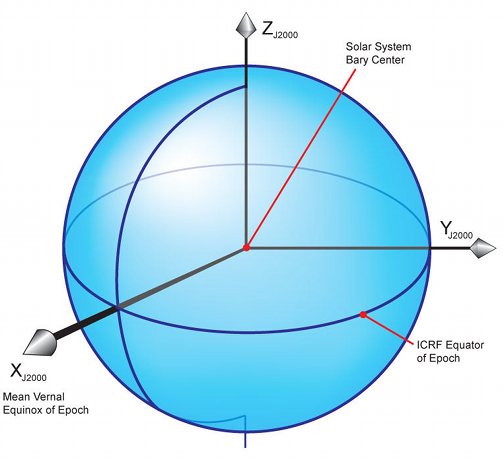
\includegraphics [width=7in]{figs/fig1.png}
\caption{The ICRF and BCRF System}
\label{fig:1}
\end{figure}

\subsection{ICRF and BCRF Example}
To know the position of the Sun and Moon, for example, one must set up a sim\_object in the S\_define file , for instance in SIM 4 in the \hyperTutorial. Let the JPL ephemerides be DE421. The entry is then:
\begin{verbatim}
environment/ephemerides/de4xx_ephem:  De4xxEphemeris de421
      (environment/ephemerides/de4xx_ephem/data/de421.d);
\end{verbatim}
In this example the multibody gravitational forces from the Sun and Moon need to be invoked. In the Modified Data directory for Tutorial Sim 4 the following lines should be set:

\begin{verbatim}
/* Set up the gravity controls for the Sun. */
VEH_OBJ.sun_grav_ctrl.planet_name   = "Sun";
VEH_OBJ.sun_grav_ctrl.active        = True;
VEH_OBJ.sun_grav_ctrl.spherical     = True;

/* Set up the gravity controls for the Moon. */
VEH_OBJ.moon_grav_ctrl.planet_name  = "Moon";
VEH_OBJ.moon_grav_ctrl.active       = True;
VEH_OBJ.moon_grav_ctrl.spherical    = True;
\end{verbatim}


